% !TeX spellcheck = de_CH_frami
\newpage
\section{Gebräuchliche Realisierung von OTA's (Kap. 14)}
Ein einstufiger OTA wird bereits durch eine Differenzstufe realisiert.
In der Praxis wird ein OTA aber nie so realisiert, da eine Last am Ausgang die Symmetrie der Differenzstufe stört.\\[2ex]
\begin{minipage}[t]{0.25\textwidth}
	\textbf{Symmetrischer OTA}\\
	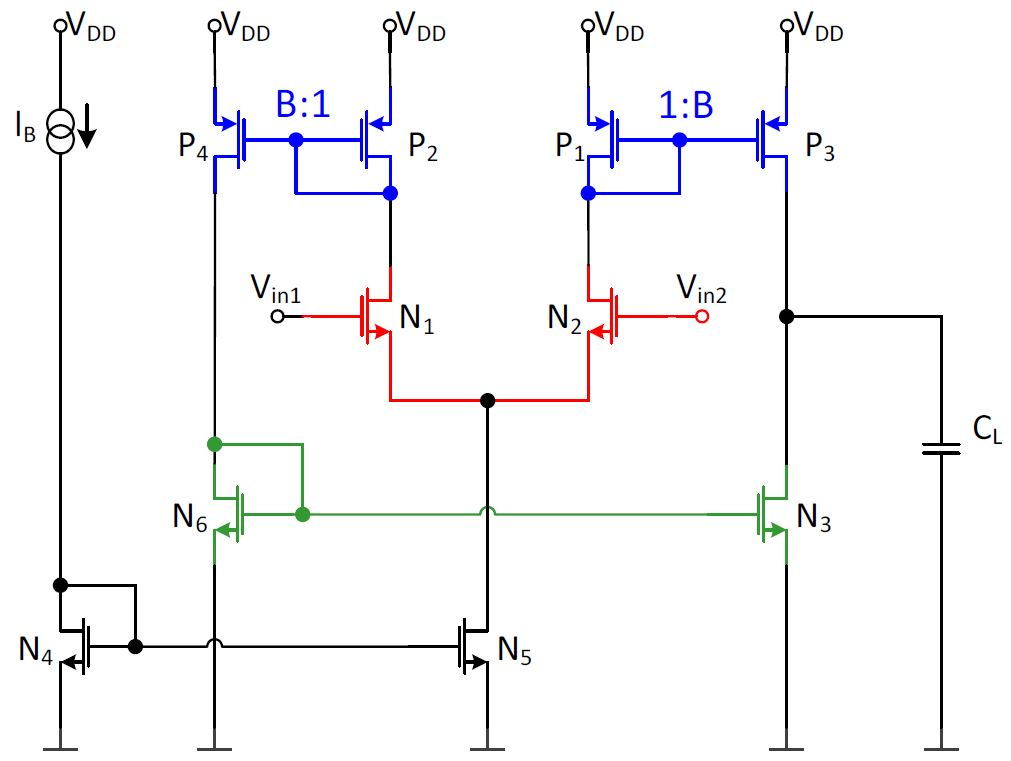
\includegraphics[width=1\linewidth]{chapters/OTA/images/SymmetrischerOTA}\\
\end{minipage}
\begin{minipage}[t]{0.25\textwidth}
	\textbf{Telescopic cascode OTA}\\
	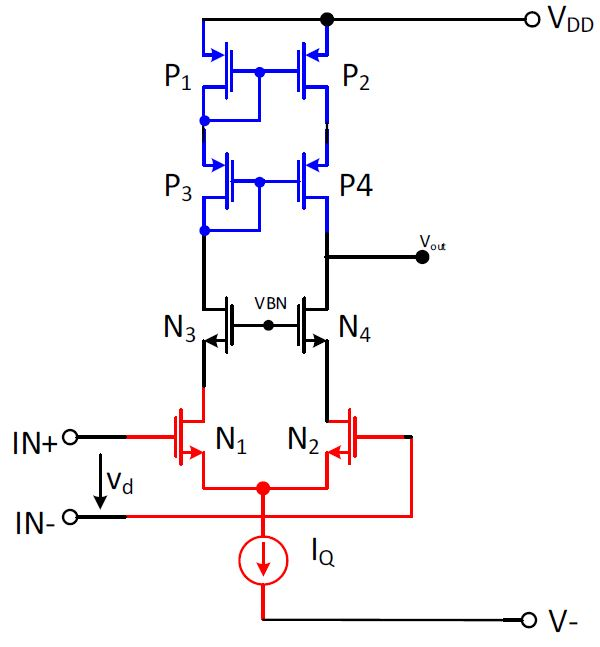
\includegraphics[width=0.7\linewidth]{chapters/OTA/images/TelescopicCascodeOTA}\\
\end{minipage}
\begin{minipage}[t]{0.5\textwidth}
	\textbf{Folded cascode OTA}\\
	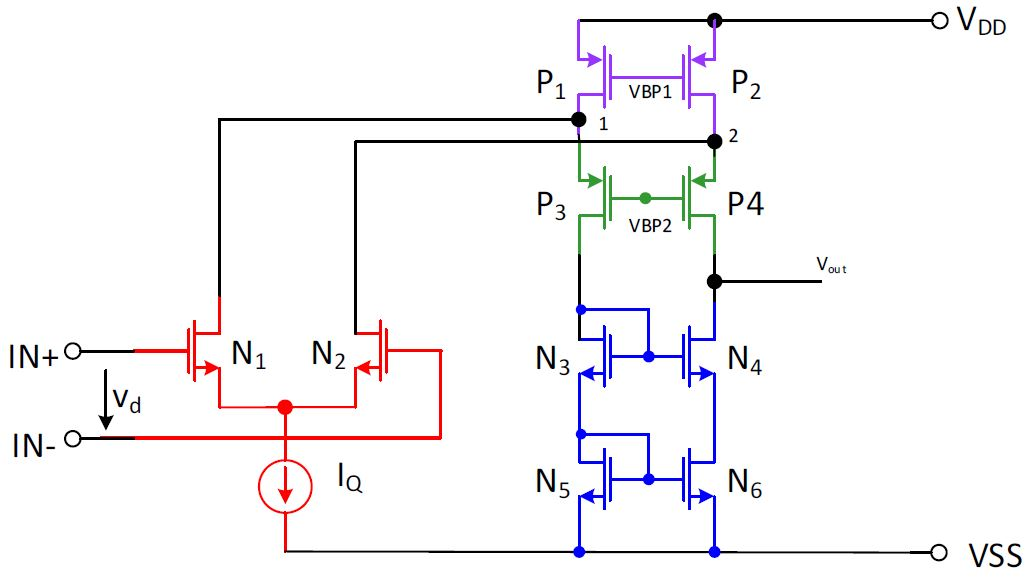
\includegraphics[width=0.7\linewidth]{chapters/OTA/images/FoldedCascodeOTA}\\
\end{minipage}\\
\begin{tabular}{|l|p{3cm}|l|l|l|p{3cm}|}
	\hline
	OTA-Typ&$a$&$r_{out}$&$BW$&$GBW$&Bemerkung\\ \hline
	Symmetrischer OTA&$B\cdot g_{m\_N1}\cdot r_{out}$&$(r_{DS\_N3}||r_{DS\_P3})$&$\frac{1}{2\pi\cdot r_{out}C_L}$&$B\cdot\frac{g_{m\_N1}}{2\pi\cdot C_L}$& \\ \hline
	Telescopic Cascode&$-g_{mN1,N2} \cdot r_{out}$&$(r_{K\_N}||r_{K\_P})$&$\frac{1}{2\pi\cdot r_{out}C_L}$&$\frac{g_{m\_N1,2}}{2\pi C_L}$&$r_{K\_N,K\_P}\approx r_{DS}\cdot(2+g_m\cdot r_{DS})$\\ \hline
	Folded Cascode&$g_{mN1,N2}\cdot r_{out}$&$(r_{K\_N}||r_{K\_P})$&$\frac{1}{2\pi\cdot r_{out}C_L}$&$\frac{g_{m\_N1,2}}{2\pi\cdot C_L}$&\\ \hline
	
\end{tabular}\\[2ex]
\textbf{Miller OTA - Designgleichungen}\\
\begin{minipage}[t]{0.3\textwidth}
	Schaltung:\\
	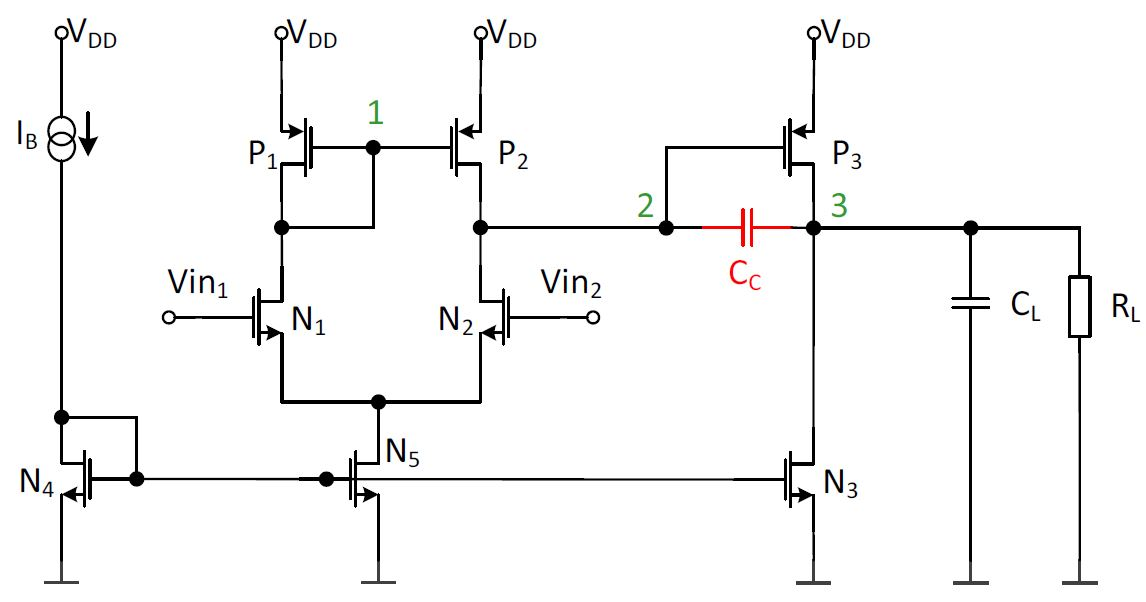
\includegraphics[width=1\linewidth]{chapters/OTA/images/MillerOTA}
\end{minipage}
\begin{minipage}[t]{0.7\textwidth}
	Wichtige Parameter:\\
	\begin{tabular}{|l|l|}
		\hline
		Dominanter Pol:&$f_{pN2}=\frac{1}{2\pi R_{N2}(C_{N2}+a_2C_c)}\approx\frac{1}{2\pi R_{N2}a_2C_c}$\\ \hline
		Nondominanter Pol:&$f_{Nd}=f_{N3}=\frac{1}{2\pi R_{N3}C_L}\approx\frac{g_{mP3}}{2\pi C_L}$\\ \hline
		3dB Bandbreite:&$BW\approx f_d=f_{N2}=\frac{1}{2\pi R_{N2}a_2C_c}$\\ \hline
		Phasenmarge:&$\varphi_M =\SI{90}{\degree}-arctan(\frac{GBW}{f_{nd}})$\\ \hline
		Gain-Bandwidth Produkt:&$GBP=a\cdot f_d=\frac{g_{mN1,2}R_{N2}\cdot g_{mP3}R_{N3}}{2\pi R_{N2}a_2C_c}=\frac{g_{mN1}}{2\pi C_c}$\\ \hline
		Nullstelle:&$f_z\approx\frac{g_{mP3}}{2\pi C_c}$\\ \hline
		Verstärkung:&$a=a_1\cdot a_2=g_{mN1,2}R_{N2}\cdot g_{mP3}R_{N3}=$\\
		&$g_{mN1,2}(r_{DS\_N2}||r_{DS\_P2})\cdot g_{mP3}(r_{DS\_N3}||r_{DS\_N3}||R_L)$\\ \hline
	\end{tabular}
\end{minipage}
